\chapter{Results} \label{results}
%\begin{figure}[H]
%\centering
%    \begin{minipage}{0.45\textwidth}
%%        \centering
%        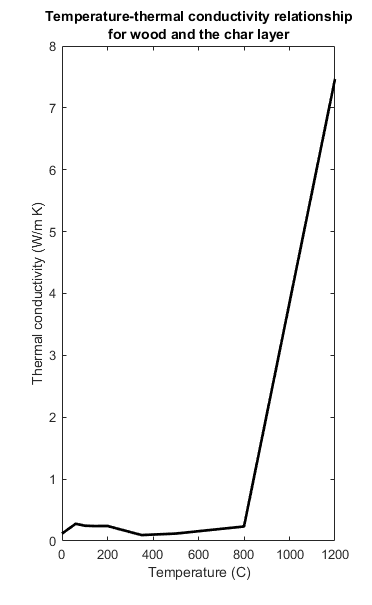
\includegraphics[width=0.9\textwidth]{figures/resultsk_cropped.png} % first figure itself
%        \caption{The resulting $\kappa$-values }
%        \label{kresult_fig}
%    \end{minipage}
%    \begin{minipage}{0.45\textwidth}
%%        \centering
%        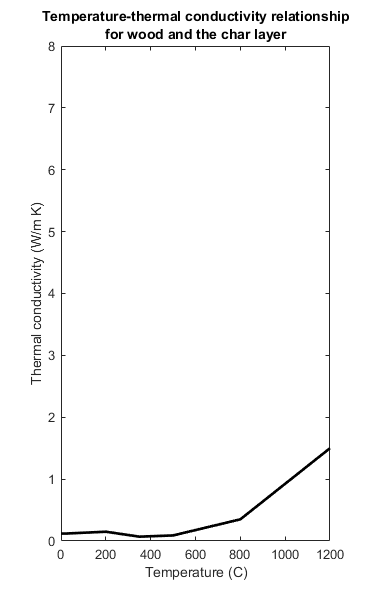
\includegraphics[width=0.9\textwidth]{figures/eurok_samescale_cropped.png} % second figure itself
%        \caption{The original $\kappa$-values}
%        \label{scalekeuro_fig}
%    \end{minipage}
%\end{figure}\

The results of running the algorithm until 20 000 acceptable values are found is shown below.)TODO add more.
\section{Resulting k-values}
The thermal diffusivity ($\kappa$-values) at key temperatures was the main goal of this project. 
As can be seen in Figure \ref{kresult_euro_fig} there was quite a drastic difference in the thermal diffusivity at 1200 $^{^\circ}$C and between 0$^{^\circ}$C and 200$^{^\circ}$C.
thee large difference at 1200$^{^\circ}$C is due to how our model is created.(TODO?)
Most of the energy at that temperature is radiated?(TODO)
\begin{figure}[H]
	\label{kresult_euro_fig}
	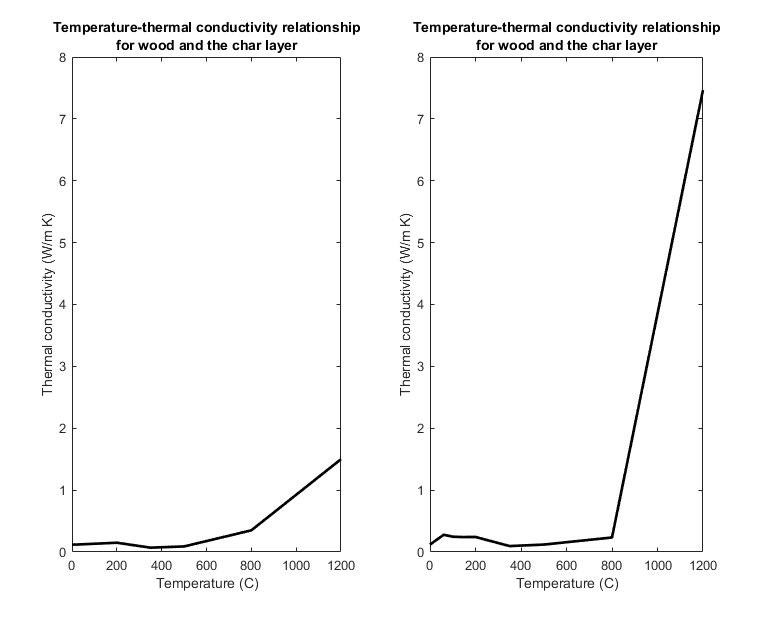
\includegraphics[width=\linewidth]{figures/euro_and_results.png}
	\caption{Resulting $\kappa$ values (left) compared to Euro-code standard values(right)}
\end{figure}


\section{Model output}
In Figure \ref{data_newk} the difference in output from running the model with the new $\kappa$ values, Euro code $\kappa$ and the measured data can be seen. 

\begin{figure}[H]
	\label{data_newk}
	\centering
	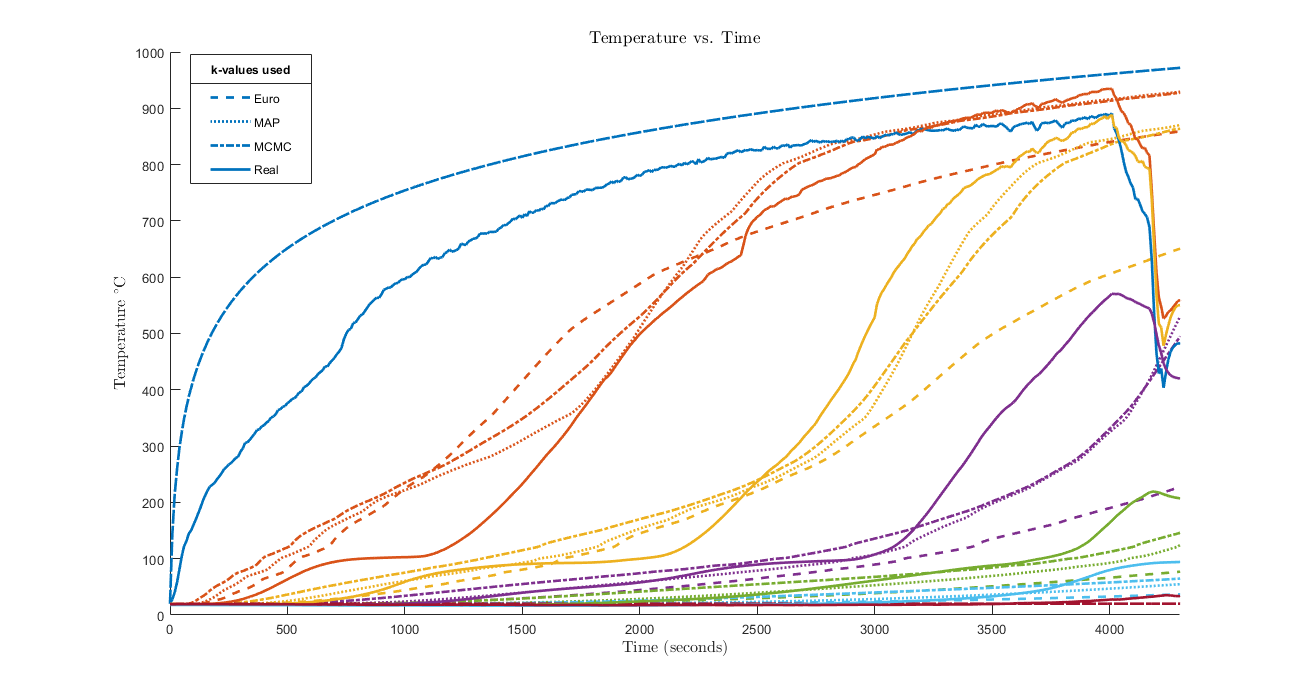
\includegraphics[width=\linewidth,]{figures/final_graph.png}
\end{figure}
